\chapter{Application examples}
\label{chap:ApplicationExamples}
%
\section{Comparison of different tuning methods from a multi-objective frame}
La idea acá es comparar algunos métodos y ver cómo terminan puestos en el Pareto
%
\section{High order benchmark plant}
\label{sec:Bechmark}
To do
%
\section{LiTaO$_3$ Thin Film Deposition Process}
\label{sec:LiTAO3}
Temperature control is a very important factor in the deposition process of lithium tantalate (LiTaO$_3$) by means of metal organic chemical vapor deposition (MOCVD) \cite{Zhang2004}.


The dynamics of the reactor chamber are characterized by a large lag and time-delay. It is important for the quality of the final product, that the controller follow a predefined temperature profile accurately (servo control) while been able to reject other disturbances (regulatory control).

The model of the MOCVD chamber can be given by:
\begin{equation}
G(s) = \frac{K e^{-L s}}{T s+1},
\label{eq:GsLita}
\end{equation}
%
where the gain $K = 3.2$, the time constant $T = 200$~s and the time-delay $L = 150$~s.

For this case, a two function MOOP is considered with $J_{di}$ and $J_{r}$ as cost functions and a robustness restriction of $M_S = 2.0$. When solving the optimization using the ENNC method, the obtained Pareto front is as given in %
\begin{figure}
	\centering
	\begin{tikzpicture}
	\begin{axis}[
	xlabel = $J_{di}$,
	ylabel = $J_{r}$,
	grid = major,
	width=0.8\columnwidth,
	xtick={0.7,0.75,...,1.2},
	ytick={1.2,1.22,...,1.5},
	]
	\addplot[mark=none, line width=2pt,] table[x=Jdi, y=Jr]{./tablas/Pareto_LiTa_ms2.dat};
	\end{axis}
	\end{tikzpicture}
	\caption{Pareto front for the LiTaO$_3$ thin film deposition process.}
	\label{fig:LitaPareto}
\end{figure}
%
figure~\ref{fig:LitaPareto}. In this case, the Pareto front is fairly convex.
%
\section{Continuous stirred tank heater}
\label{sec:CSTH}
%
The control of a \gls{csth} is a common task in industrial processes. In this section, the control of the temperature of the \gls{csth} will be solved as a \gls{moop} using a \gls{2dof} \gls{pid} controller. The diagram of the process is presented in %
\begin{figure}[b]
	\centering
	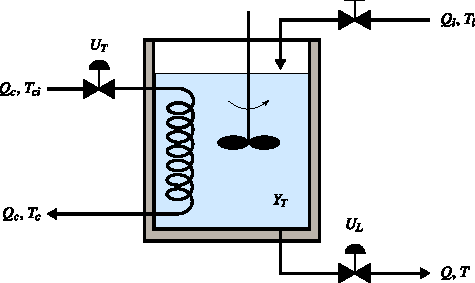
\includegraphics{Ch7CSTR}
	\caption{Simplified diagram of a continuous stirred-tank heater to be controlled.}
	\label{fig:Ch7CSTR}
\end{figure}
Figure~\ref{fig:Ch7CSTR}. A heat exchanger is installed inside the tank to heat the fluid. The flow rate inside the heat exchanger is controlled with a valve with input variable $U_T$ and the liquid inside the heat exchanger enters with temperature $T_{ci}$ and leaves with temperature $T_{co}$. The volume inside the tank is variable, the input flow rate is $Q_i$ with temperature $T_i$. The output flow rate is $Q$ with temperature $T$. The output flow rate is controlled with a valve with input variable $U_L$. The tank is covered with a jacket that prevents any heat loss to the atmosphere.

According to \cite{Alfaro2016}, a possible model for this process is given by the following set of algebraic-differential equations:
\begin{itemize}
	\item Tank mass balance:
			\begin{equation*}
				A \frac{d H(t)}{dt} = Q_i(t) - Q(t),
			\end{equation*}
			where $A$ is the transversal area of the tank and $H(t)$ is the liquid level.
	\item Tank energy balance:
			\begin{equation*}
				\rho C_p A H(t) \frac{T(t)}{dt} = \rho C_p Q_i(t)\left( T_i(t) - T(t)\right) + W(t),
			\end{equation*}
			where $C_p$ is the heat capacity of the fluid and $W(t)$ is the rate of heat transfer from the heat exchanger to the tank. $W(t)$ can be modeled as:
	\item Heat exchanger energy balance:
			\begin{equation*}
				\rho_c C_{pc} V_c \frac{T_{co}}{dt} = \rho_c C_{pc} Q_c(t)\left( T_{ci}-T_{co}\right) - W(t),
			\end{equation*}
			where $\rho_c$ is the density of the fluid inside the heat exchanger, $C_{pc}$ is the heat capacity of the fluid inside the heat exchanger and $V_c$ is the volume of the heat exchanger.
	\item Heat transfer between the heat exchanger and the fluid in the tank:
			\begin{equation*}
				W(t) = U A_c \left( T_{ca}(t) - T(t)\right), 
			\end{equation*}
			where $U$ is overall heat-transfer coefficient, $A_c$ is the area of the heat exchanger, $T_{ca}$ is the average temperature inside the heat exchanger given by:
			\begin{equation*}
				T_{ca}(t) = \frac{T_{ci}(t) + T_{co}(t)}{2}
			\end{equation*}
\end{itemize}

Also, in \cite{Alfaro2016}, the transmitters and the valves are modeled as:
\begin{itemize}
	\item Level transmitter: it is supposed that the level transmitter is a capacitive type electronic transmitter that has a first order dynamics:
		\begin{equation*}
			T_L \frac{d Y_L(t)}{dt} + Y_L(t) = K_L H(t),
		\end{equation*}
		%
		where $T_L$ is its time constant, $Y_L$ is the level signal and $K_L$ is the transmitter gain.
	%
	\item Temperature transmitter: It is supposed that a Pt$_{100}$ RTD electronic sensor is installed in a thermowell at the tank outlet pipe. It is supposed that it has a second order dynamic:
	%
		\begin{equation*}
			T_{T}^2 \frac{d^2 Y_T(t)}{dt^2} + 2T_T \frac{d Y_T(t)}{dt} + Y_T(t) = K_T T(t),
		\end{equation*}
		%
		where $T_T$ is its time constant and $K_T$ is its gain.
	%
	\item Level control valve: it is supposed that a ball valve with an electroneumatic actuator is used. The valve	inherent flow characteristics is nearly quadratic and the relationship between the flow $Q(t)$ and the input variable $U_L$ is given by:
		\begin{align*}
			T_{vL} \frac{d X_L(t)}{dt} + X_L(t) = K_{xL} U_L(t),\\
			Q(t) = K_{vL} X_L^2(t)\sqrt{\rho g H(t)},
		\end{align*}
		where $T_{vL}$ is the level control valve time constant, $K_{xL}$ level control valve stem constant $K_{vL}$ level control valve constant and $X_L(t)$ is the level control valve stem normalized travel.
	%
	\item Temperature control valve it is also supposed to be a ball valve with an electroneumatic actuator, however, it is supposed that the valve has an equal-percentage inherent flow characteristics given by:
		\begin{align*}
			T_{vT} \frac{d X_T(t)}{dt} + X_T(t) = K_{xT} U_T(t),\\
			Q_c(t) = K_{vT}R_{vT}^{\left( X_T(t) -1 \right) } \sqrt{P_{cp} - \left(R_c Q^2_c(t)+P_{cr} \right) },
		\end{align*}
		where $T_{vT}$ is the temperature control valve time constant, $K_{xT}$ the temperature control valve stem constant, $K_{vT}$ is the temperature control valve constant $P_{cp}$ is the heating fluid pump discharge pressure, $P_{cr}$ is heating fluid system return pressure and $X_T(t)$ is the temperature control valve stem normalized travel.
\end{itemize}

Taking this model in consideration, it can be said that, from the point of view of the controller, the controlled variables are give by the signals $Y_L(t)$ (which represents the level) and $Y_T(t)$ (which represents the temperature of the fluid of the tank). The manipulated variables are given by $U_L(t)$ (which directly affects $Q$) and $U_T(t)$ (that directly affects $Q_{c}$). $Q_i(t)$, $T_i$ and $T_{ci}$ are considered as disturbances. The state variables of the system are given by $H(t)$, $T_T(t)$, $T_{co}$, $Y_L(t)$, $Y_T$, $X_L(t)$ and $X_T(t)$, therefore, this model comprises a seventh order non-linear system for a two-input two-output industrial process.